\documentclass{article}
\usepackage[utf8]{inputenc}
\usepackage[english]{babel}
\usepackage[table]{xcolor}
\usepackage{siunitx}
\usepackage{geometry}
\usepackage{graphicx}
\usepackage{longtable}
\usepackage{booktabs}
\usepackage{amsmath}
\usepackage{amssymb}
\usepackage{array}
\geometry{
  left=0.5in,
  top=0.2in,
  right=0.5in,
  bottom=0.5in
}
\sisetup{
  round-mode=places, % Rounds numbers
  round-precision=2, % to 2 places
}
\graphicspath{{./images/}} % image path
\definecolor{R}{HTML}{6495ed} % cornflowerblue
\definecolor{G}{HTML}{20b2aa} % lightseagreen
\definecolor{B}{HTML}{cd5c5c} % indianred
\definecolor{A}{HTML}{663399} % rebeccapurple
\def\BOX#1#2{\bf\textcolor{#2}{#1}}
\def\TEMPERATURE#1{\textbf{#1}}
\def\MG{\scriptstyle{mg/cm^2}}
\def\PM{\textcolor{black}{\pm}}
\def\I#1#2#3{\hspace*{#2}\textbf{#1}\hspace*{#3}}
\def\TC{\(\left(\vcenter{\hbox{\(\scriptstyle{\text{\textdegree{C}}}\)}}\right)\)\hspace*{3em}}
\def\WT#1#2{\hspace*{#1}\(\left(\vcenter{\hbox{\(\scriptstyle{mg/cm^2}\)}}\right)\)\hspace*{#2}}
\def\ONE{\bf\textcolor{R}{26}}
\def\TWO{\bf\textcolor{G}{28}}
\def\THR{\bf\textcolor{B}{30}}
\def\FOR{\bf\textcolor{A}{26\text{-}30}}
\def\C{\(\scriptstyle{\text{\textdegree{C}}}\)}
\def\RONE{\(\ONE\scriptstyle{\text{\textdegree{C}}}_{\{\BOX{01}{R} - \BOX{11}{R}\}}\)}
\def\RTWO{\(\TWO\scriptstyle{\text{\textdegree{C}}}_{\{\BOX{12}{G} - \BOX{21}{G}\}}\)}
\def\RTHR{\(\THR\scriptstyle{\text{\textdegree{C}}}_{\{\BOX{22}{B} - \BOX{30}{B}\}}\)}
\def\RFOR{\(\FOR\scriptstyle{\text{\textdegree{C}}}_{\{\BOX{31}{G} - \BOX{41}{A}\}}\)}
\def\MEAN#1#2#3#4{\(\tfrac{C_{\BOX{#2}{#1}}+\cdots+C_{\BOX{#3}{#1}}}{\BOX{#4}{#1}}\)}
\def\STD#1#2#3#4{\(\sqrt{\tfrac{\left|C_{\BOX{#2}{#1}} -\overline{C}\right|^2+\cdots+\left|C_{\BOX{#3}{#1}} -\overline{C}\right|^2}{\BOX{#4}{#1} - 1}}\)}
\def\ERR#1#2#3#4{\(\tfrac{\overline{\sigma}_{\{\BOX{#2}{#1} - \BOX{#3}{#1}\}}}{\sqrt{\BOX{#4}{#1}}}\)}
% title, name, date
\title{Analysis of Coral Growth Lab Report}
\author{Philip Kim}
\date{\today}
\begin{document}
\maketitle
\vspace*{-1cm}
% Dataset Table: Treatment, Initial, Final, Change
\begin{longtable}[c]{|c|r|r|r|r|}
  \toprule
  \textbf{\#} &
  \TEMPERATURE{TREATMENT} &
  \TEMPERATURE{\textcolor{white}{TREATMENT}} &
  \TEMPERATURE{\textcolor{white}{TREATMENT}} &
  \TEMPERATURE{\textcolor{white}{TREATMENT}}\\
  &
  \TC\ &
  \WT{0em}{1.8em} &
  \WT{0em}{1.8em} &
  \WT{0em}{1.8em}\\
  \midrule\endfirsthead%

  \toprule
  \textbf{\#} &
  \TEMPERATURE{TREATMENT} &
  \TEMPERATURE{\textcolor{white}{TREATMENT}} &
  \TEMPERATURE{\textcolor{white}{TREATMENT}} &
  \TEMPERATURE{\textcolor{white}{TREATMENT}}\\
  &
  \TC\ &
  \WT{0em}{1.8em} &
  \WT{0em}{1.8em} &
  \WT{0em}{1.8em}\\
  \midrule\endhead%
    1 & \ONE\ & 552 & 563 & 11\\\midrule
    2 & \ONE\ & 341 & 352 & 11\\\midrule
    3 & \ONE\ & 461 & 467 & 6\\\midrule
    4 & \ONE\ & 430 & 437 & 7\\\midrule
    5 & \ONE\ & 312 & 320 & 8\\\midrule
    6 & \ONE\ & 364 & 374 & 10\\\midrule
    7 & \ONE\ & 468 & 479 & 11\\\midrule
    8 & \ONE\ & 449 & 460 & 11\\\midrule
    9 & \ONE\ & 398 & 415 & 17\\\midrule
    10 & \ONE\ & 394 & 401 & 7\\\midrule
    11 & \ONE\ & 360 & 369 & 9\\
  \midrule%
    12 & \TWO\ & 517 & 528 & 11\\\midrule
    13 & \TWO\ & 428 & 443 & 15\\\midrule
    14 & \TWO\ & 407 & 415 & 8\\\midrule
    15 & \TWO\ & 441 & 452 & 11\\\midrule
    16 & \TWO\ & 472 & 488 & 16\\\midrule
    17 & \TWO\ & 383 & 391 & 8\\\midrule
    18 & \TWO\ & 466 & 479 & 13\\\midrule
    19 & \TWO\ & 345 & 354 & 9\\\midrule
    20 & \TWO\ & 382 & 393 & 11\\\midrule
    21 & \TWO\ & 494 & 503 & 9\\
  \midrule%
    22 & \THR\ & 573 & 585 & 12\\\midrule
    23 & \THR\ & 354 & 369 & 15\\\midrule
    24 & \THR\ & 532 & 545 & 13\\\midrule
    25 & \THR\ & 393 & 410 & 17\\\midrule
    26 & \THR\ & 269 & 277 & 8\\\midrule
    27 & \THR\ & 517 & 526 & 9\\\midrule
    28 & \THR\ & 469 & 484 & 15\\\midrule
    29 & \THR\ & 306 & 322 & 16\\\midrule
    30 & \THR\ & 431 & 446 & 15\\
  \midrule%
    31 & \FOR\ & 306 & 312 & 6\\\midrule
    32 & \FOR\ & 372 & 378 & 6\\\midrule
    33 & \FOR\ & 333 & 344 & 11\\\midrule
    34 & \FOR\ & 567 & 578 & 11\\\midrule
    35 & \FOR\ & 379 & 392 & 13\\\midrule
    36 & \FOR\ & 490 & 505 & 15\\\midrule
    37 & \FOR\ & 391 & 401 & 10\\\midrule
    38 & \FOR\ & 509 & 523 & 14\\\midrule
    39 & \FOR\ & 369 & 377 & 8\\\midrule
    40 & \FOR\ & 337 & 351 & 14\\\midrule
    41 & \FOR\ & 365 & 373 & 8\\
  \bottomrule
\end{longtable}
\begin{center}
  \text{Sample Size, \textbf{N}}\\
  \text{Final -\ Initial, \textbf{CHANGE} (\textbf{C})}\\
  \text{Average Change, \textbf{MEAN} (\(\bf\overline{C}\))}\\
  \text{Standard Deviation, \textbf{STD} (\(\bf\sigma \))}\\
  \text{Standard Error, \textbf{ERR} (\(\bf\epsilon \))}
\end{center}
\begin{center}
  \begin{tabular}{*{4}{|c|}}\toprule
    \I{N}{0em}{0em} &\I{MEAN}{0em}{0em} &\I{STD}{0em}{0em} &\I{ERR}{0em}{0em}\\\midrule
    \RONE=~\BOX{11}{R} &\MEAN{R}{01}{11}{11}~=~\BOX{09.82}{R} &\STD{R}{01}{11}{11}~=~\BOX{03.03}{R} &\ERR{R}{01}{11}{11}~=~\BOX{~0.91}{R}\\\midrule
    \RTWO=~\BOX{10}{G} &\MEAN{G}{12}{21}{10}~=~\BOX{11.10}{G} &\STD{G}{12}{21}{10}~=~\BOX{02.81}{G} &\ERR{G}{12}{21}{10}~=~\BOX{~0.89}{G}\\\midrule
    \RTHR=~\BOX{09}{B} &\MEAN{B}{22}{30}{09}~=~\BOX{13.33}{B} &\STD{B}{22}{30}{09}~=~\BOX{03.12}{B} &\ERR{B}{22}{30}{09}~=~\BOX{~1.04}{B}\\\midrule
    \RFOR=~\BOX{11}{A} &\MEAN{A}{31}{41}{11}~=~\BOX{10.55}{A} &\STD{A}{31}{41}{11}~=~\BOX{03.24}{A} &\ERR{A}{31}{41}{11}~=~\BOX{~~.98}{A}\\\bottomrule
  \end{tabular}
  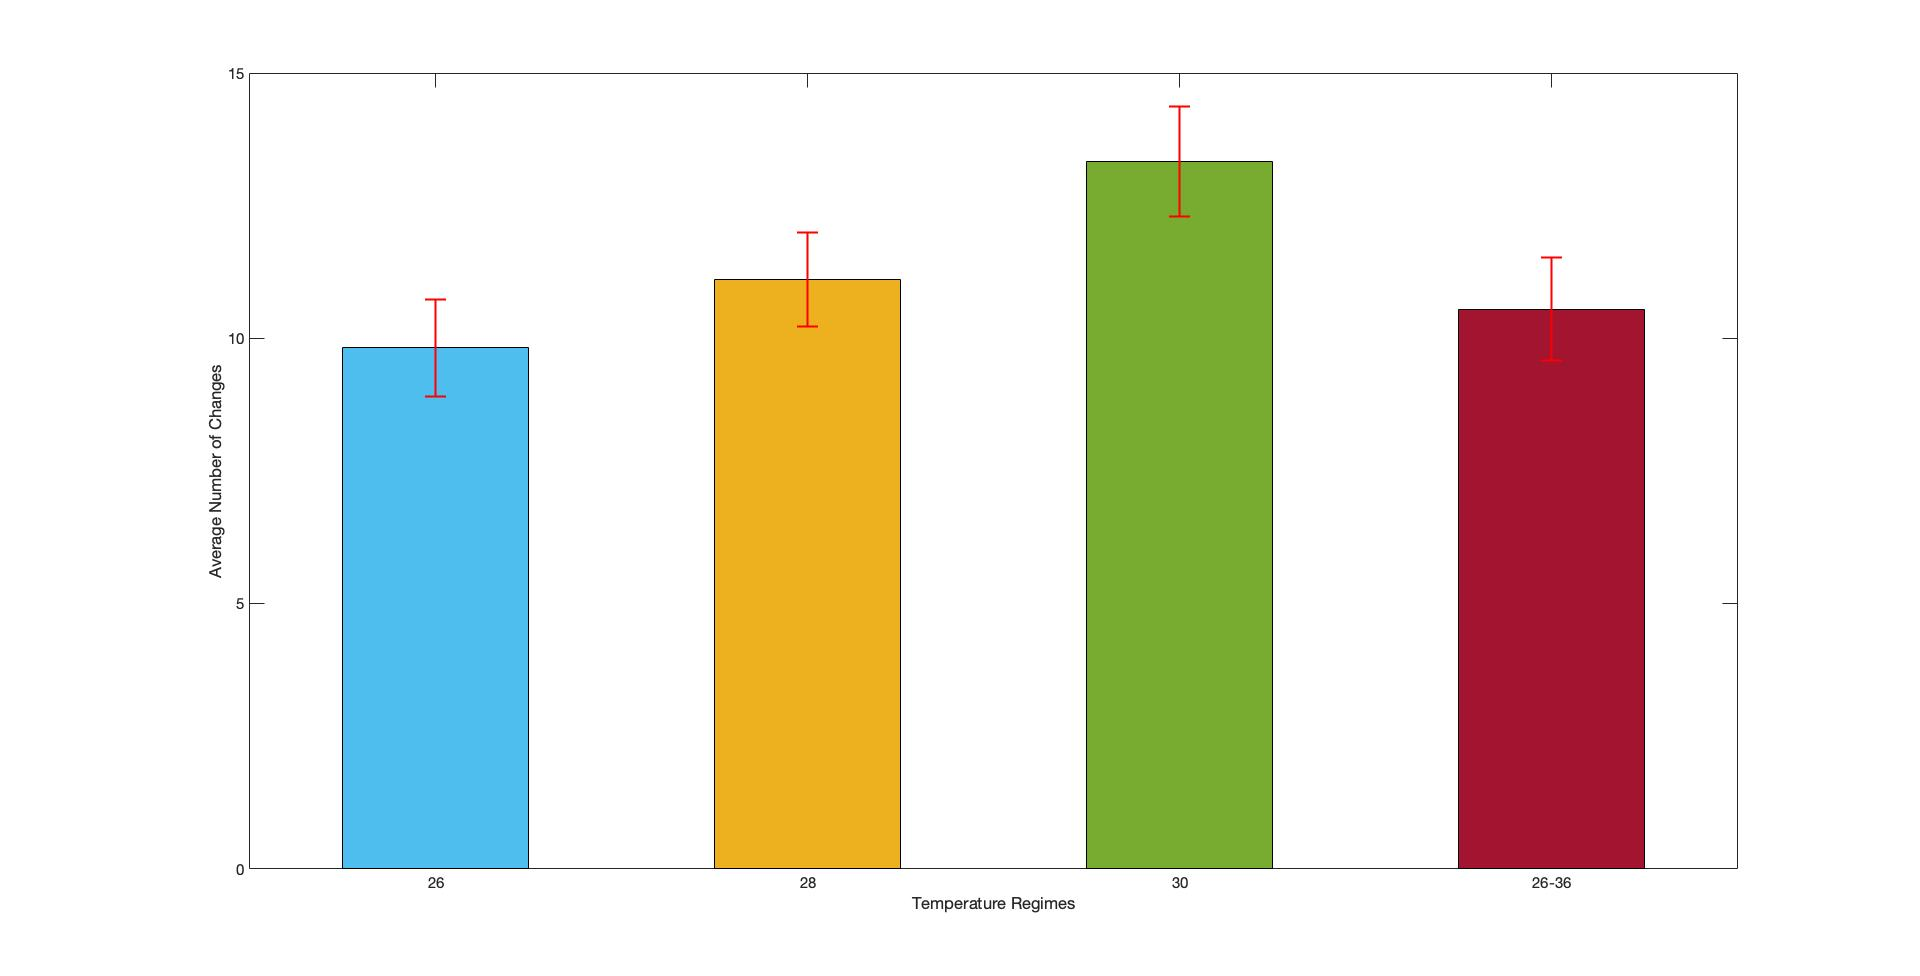
\includegraphics[width=\textwidth]{graph.jpg}
  \fbox{\begin{minipage}{53em}
    \begin{enumerate}
      \item What was the mean \(\pm \) standard error of coral growth at each of the four temperature categories?
      \item[] {\BOX{26}{R}\C~=~\BOX{\boxed{09.82~\PM0.91}}{R},
      \BOX{28}{G}\C~=~\BOX{\boxed{11.10~\PM0.84}}{G},
      \BOX{30}{B}\C~=~\BOX{\boxed{13.33~\PM1.04}}{B},
      \BOX{26\text{-}30}{A}\C~=~\BOX{\boxed{10.55~\PM0.98}}{A}}
      \item What would happen if global climate change causes the average seawater temperature to increase to 30\C?\
      \item[] By analyzing the bar graph above, {\THR\C} is significantly different with all of the temperature regimes since the error bar does not overlap with any the other temperature regimes. This means the corals growth rate at {\THR\C} is significantly the highest. If global climate change causes the average seawater to increase from {\ONE\C} to {\THR\C}, then it would be safe to assume that corals in the ocean would significantly increase.
    \end{enumerate}
  \end{minipage}}
\end{center}
\end{document}
